\documentclass[a4paper]{jpconf}
\usepackage{amsmath} % for subequations
\usepackage{xfrac} %to write fractions in different ways
\usepackage{graphicx} %for figures
\usepackage{caption} %for figures



\begin{document}

\title{The effect of solid objects on the electrostatic potential}
\author{J Cork, T  Hendrick-Beattie, D Lafferty, M Pereira, V Nordgren and N Warrack}
\address{School of Physics and Astronomy, University of Glasgow, Glasgow, UK}

\begin{abstract}
\end{abstract}

\section*{Introduction}
Electromagnetism is one of four fundamental forces of nature. It describes how electrically charged particles interact with each other and how they generate electromagnetic fields \cite{Sears.Zamansky-uniPhy}. These fields permeate the space around them, influencing the behaviour of other charges by exerting forces on them. %(that is either attractive or repulsive). 
Electromagnetic forces determine the atomic and macroscopic properties of matter that dominate most of the physical phenomena encountered in daily life such as sound, light and biological processes. Understanding these principles in depth can facilitate significant advances in science and technology. For instance, successful modelling of a simple configuration of conductors makes it possible to investigate arbitrarily complex systems of charges aiding the design of detectors for particle physics. 


%EXTRA
%The electromagnetic force plays a major role in determining the internal properties of most objects encountered in daily life. Ordinary matter takes its form as a result of intermolecular forces between individual molecules in matter. Electrons are bound by electromagnetic wave mechanics into orbitals around atomic nuclei to form atoms, which are the building blocks of molecules. This governs the processes involved in chemistry, which arise from interactions between the electrons of neighboring atoms, which are in turn determined by the interaction between electromagnetic force and the momentum of the electrons.

Electrostatics is the study of stationary or slow-moving electric charges \cite{griffiths-introElec}. They exert electrostatic forces on each other, which in turn are governed by Coulomb's law and most conveniently described by electric field equations. The relationship between these fields and the distribution of electric charge can be expressed as \cite{griffiths-introElec}
\begin{equation}
\textbf{$\nabla$} \cdot \textbf{E} = \frac{\rho}{\epsilon_0}~,
%\oint \textbf{E} \cdot d\textbf{A} = \frac{Q_{enc}}{\epsilon_0}
\label{eq:intro1}
\end{equation} known as the differential form of Guass's law, where \textbf{$\nabla$} $\cdot$ \textbf{E} is the divergence of the electric field, $\epsilon_0$ is the permittivity of free space and $\rho$ is the charge density. Additionally, for any static charge distribution the electric field is irrotational, \textbf{$\nabla$} $\times$ \textbf{E} $= 0$. Therefore, the line integral of the electric field, $\oint \textbf{E} \cdot d \textbf{l} = 0$, is independent of the path taken \cite{griffiths-introElec}. This means that \textbf{E} can be written as the gradient of a scalar potential 
\begin{equation}
\textbf{E} = - \nabla \Phi~,
\label{eq:intro2}
\end{equation} where $\Phi$ is called the electric potential, defined as the potential energy per unit charge  \cite{Sears.Zamansky-uniPhy}.
In regions where there is no charge, such that $\rho = 0$, the divergence of the electric field is zero. Hence, using Eq.(\ref{eq:intro1}) and Eq.(\ref{eq:intro2}) the electric potential for any point in space can be described by
\begin{equation}
\nabla^2 \Phi = 0~.
\label{eq:intro3}
\end{equation} This is Laplace's equation \cite{RHB-MathematicalMethods}.\\ \par
In this work, the electrostatic potential and the electric field are evaluated at all points in two different systems. The systems consist of different geometric configurations of conductors held at constant potentials. This study shows how the potentials are modified in the presence of these conductors. 

\section*{Methods}
In general, there are two methods to analyse the electric potential in all space: analytical and numerical techniques. Often there is no analytical solution, even for a simple electrostatic system, and thus numerical methods are useful tools in obtaining approximate solutions. 

\subsection*{Analytical Approach} 
%Partial differential equations (PDE) are fundamental to describe physical phenomena, such as heat, fluids, electrostatics, sound and so on. This is an equation that involves an unknown function of two or more variables and their partial derivatives. A particular solution may be specified from the general solution of a PDE in the presence of boundary conditions. \par

The electric field is dominated by inherent symmetries that are better described in spherical coordinates \cite{RHB-MathematicalMethods} in which Laplace's Equation is expressed as

\begin{equation}
\frac{1}{r^2}\frac{\partial}{\partial r}\bigg(r^2 \frac{\partial \Phi}{\partial r}\bigg) + \frac{1}{r^2 \sin \theta} \frac{\partial}{\partial \theta}\bigg(\sin \theta \frac{\partial \Phi}{\partial \theta}\bigg) + \frac{1}{r^2 \sin^2 \theta}\frac{\partial^2 \Phi}{\partial \phi^2} = 0~.
\label{eq:1}
\end{equation}

For round objects $\Phi$ can be independent of $\phi$ given an appropriate choice of coordinate orientation. Multiplying through by $r^2$ the equation is simplified to
\begin{equation}
\frac{\partial}{\partial r}\bigg(r^2 \frac{\partial \Phi}{\partial r}\bigg) + \frac{1}{\sin \theta}\frac{\partial}{\partial \theta}\bigg(\sin \theta \frac{\partial \Phi}{\partial \theta}\bigg) = 0~.
\label{eq:2}
\end{equation}

Separation of variables is used to solve the equation above. Assume that $\Phi(r,\theta) = R(r)\Theta(\theta)$, where the factors $R$ and $\Theta$ are functions of $r$ and $\theta$ respectively. Substituting for and dividing through by $\Phi$, Eq.(\ref{eq:2}) can be written as 
\begin{equation}
\frac{1}{R}\frac{d}{dr}\bigg(r^2 \frac{dR}{dr}\bigg) + \frac{1}{\Theta \sin \theta}\frac{d}{d \theta}\bigg(\sin \theta \frac{d \Theta }{d \theta}\bigg) = 0~.
\label{eq:3}
\end{equation}This form shows that the first term depends only on $r$, and the second only on $\theta$. It follows that  each term is equal to a constant defined, for convenience, to be $s(s+1)$:
\begin{subequations}
\begin{align}
&\frac{d}{dr}\bigg(r^2 \frac{dR}{dr}\bigg) = s (s+1) R~, \label{eq:4.1}\\ 
&\frac{d}{d \theta}\bigg(\sin \theta \frac{d \Theta}{d \theta}\bigg) = - s (s+1) \Theta \sin \theta~. \label{eq:4.2}
\end{align}
\label{eq:4}
\end{subequations} 

The partial differential equation, Eq.(\ref{eq:2}), has been converted into two independent ordinary differential equations. The general solution for the radial equation, Eq.(\ref{eq:4.1}), is:
\begin{equation}
R = Ar^5 + \frac{B}{r^{s+1}},
\end{equation} where $A$ and $B$ are arbitrary constants \cite{RHB-MathematicalMethods}. However, the general solution for the angular equation, Eq.(\ref{eq:4.2}), requires Legendre Polynomials in the variable $\cos \theta$. These are special functions usually encountered in physical problems involving Laplace's equation \cite{RHB-MathematicalMethods}. The solution has the form
\begin{equation}
\Theta(\theta) = P_{s}(\cos \theta)~,
\label{eq:5}
\end{equation} where $P_s$ is the $s$th-order polynomial in $x$ and can be expressed using the Rodrigues' formula \cite{RHB-MathematicalMethods}
\begin{equation}
P_s(x) = \frac{1}{2^s s!} \frac{d^s}{dx^s}(x^2 -1)^s~.
\label{eq:6}
\end{equation}

\noindent Therefore, the most general separable solution is:
\begin{equation}
\Phi(r, \theta) = \bigg(A r^s + \frac{B}{r^{s+1}}\bigg) P_s (\cos \theta)~.
\label{eq:7}
\end{equation}  

\noindent Since Laplace's equation is a linear PDE, the general solution is a superposition of all solutions corresponding to different allowed values of $s$ \cite{griffiths-introElec}. The linear combination can be written as:
\begin{equation}
\Phi(r, \theta) = \sum_{s=0}^{\infty} \bigg( A_s r^s + \frac{B_s}{r^{s+1}}\bigg) P_s (\cos \theta)~,
\label{eq:8}
\end{equation} where $A_s$ and $B_s$ are arbitrary constants that are determined by boundary conditions. \\ \par 

\subsection*{Numerical Techniques}
%\cite{Press.T.V.F-NumericalRecipes}
%Laplace?s equation is mathematically described as an elliptic PDE due to its characteristics. To find a particular solution for this differential equation additional conditions must be imposed. These conditions are boundary values that describe all or part of the perimeter of the region in which a solution is desired. The nature of these boundary conditions usually determines the numerical method required to obtain an approximate solution [4]. This is called a Boundary value problem, specifically an Elliptic boundary value problem which does not involve a time variable.

To find a particular solution for a differential equation additional conditions must be imposed, boundary values that describe all or part of the region in which the solution is desired. The nature of these boundary conditions usually determines the numerical method required to obtain an approximate solution \cite{Cheney.Kincai-NumericalMethods}. \par
Laplace's equation is mathematically described as an elliptic PDE due to its characteristics and these are fundamental for its physical significance \cite{RHB-MathematicalMethods}. Problems that are governed by elliptic PDEs and subjected to boundary conditions are called Boundary value problems.
These problems can be solved by the Finite-difference and Relaxation methods. \par

The first step of the numerical technique is to discretize the problem by defining a mesh, which is a grid of  spatial points that covers the domain of interest. The points that lie on the mesh can be written in cartesian coordinates as 
\begin{subequations}
\begin{align}
&x_i = ih\\ 
&y_j = jh
\end{align}
\label{eq:coord}
\end{subequations} 
\noindent where h is the distance between the grid points and i,j is an integer pair of indices which count grid points from some reference point. The differential operator $\nabla^2$ is then approximated 
to a discrete form through the use of finite-differences. The standard formula for second derivatives is 
\begin{equation}
f''(x) \approx \frac{1}{h^2}[f(x+h) - 2f(x) + f(x-h)].
\end{equation}
\noindent Since there are two variables, $x$ and $y$, the discrete approximation to the the Laplacian can be written as
\begin{equation}
\nabla^2 \Phi \approx \frac{\Phi(x+h,y) + \Phi(x-h,y) - 2\Phi(x,y)}{h^2} + \frac{\Phi(x,y+h) + \Phi(x,y-h) - 2\Phi(x,y)}{h^2}~,
\end{equation}
\noindent or in grid notation
\begin{equation}
(\nabla^2 \Phi)_{ij} \approx \frac{1}{h^2}[\Phi_{i+1,j} + \Phi_{i-1,j} + \Phi_{i,j+1} + \Phi_{i,j-1} - 4\Phi_{ij}]~.
\label{eq:fivepoint}
\end{equation}
This equation is called the Five-point formula. The name comes from the fact that it involves values of $\Phi$ at $(x,y)$ and at the four nearest grid points. $(\nabla^2 \Phi)_{ij}$ = 0 therefore Eq.(\ref{eq:fivepoint}) can be rewritten as 
\begin{equation}
\Phi_{i,j} = \frac{1}{4}(\Phi_{i+1,j} + \Phi_{i-1,j} + \Phi_{i,j+1} + \Phi_{i,j-1})~.
\end{equation}
\noindent This form shows that a solution to Laplace's equation has the property that at any point it is equal to the average of the values at neighbouring points \cite{Cheney.Kincai-NumericalMethods}. 

The boundary conditions are specified in the mesh and the interior points of the region desired are assigned to an arbitrary value. This value chosen will not influence the final solution but it may affect the convergence of the scheme.

The iterative scheme to solve Laplace's equation starts by guessing a solution and then sweeps across the grid updating the value at each point. On each interaction $\Phi_{i,j}$ is set to the average of the four nearest points. Initially the result will not be exact since the neighbours also get updated, but by repeating the process several times the scheme converges to a solution. When the change between iterations is two small, according to a specified error tolerance, a solution is obtained. This procedure is called Relaxation Method. This method is generally slow but others such as Jacobi or Gauss-Seidel can be implemented in order to improve it.

The inherent error in the Five-point formula is 
\begin{equation}
\frac{-h^2}{12}\bigg[\frac{\partial^4 \Phi}{\partial x^4}(\xi, y) + \frac{\partial^4 \Phi}{\partial y^4}(x,\eta)\bigg]~,
\end{equation}
\noindent which provides an approximation of order $\mathcal{O}(h^2)$ \cite{Cheney.Kincai-NumericalMethods}. The accuracy of the approximation improves as the mesh points increases, that is, as h approaches zero.  This can be done by implementing Adaptive meshing. The problem is solved using the Relaxation method on a uniform mesh and then the solution is examined to see where more gride points can be added. The procedure is then repeated with the improved mesh. This numerical technique decreases the uncertainty in the solution.


\section*{Solving a physical system}
There are simple electrostatic systems for which an analytical solution can be derived. These systems can be extremely helpful when developing a numerical solution. They are used to ensure the correctness and the accuracy of the numerical approximation. System $A$, shown in Fig.\ref{fig:systemA}, was used to obtain this information. This system has a perfectly uniform electric field defined by two plates at potential $+V$ and $-V$. %A long conducting cylinder is placed into the field at ground potential between the plates. 

\begin{figure}[h]
	\centering
	\includegraphics[width=5.7cm]{GPdiagram11} 
	\caption{CAPTION!!}
	\label{fig:systemA}
\end{figure}

When the uncharged cylindrical conductor is placed in the system the electric field is altered. The field pushes free positive charges to the right and the negative ones to the left. The charges accumulate in the edges of the conductor distorting the field in the surroundings of the cylinder. The potential outside the conductor can be described mathematically using principles of electrostatics, namely Laplace's Equation Eq.(\ref{eq:intro3}). %This PDE describes the electrostatic potential for a given charge distribution, and consequently the corresponding field. 
A particular solution defining System $A$ is obtained using Eq.(\ref{eq:8}) and the required boundary conditions. 


The potential at the surface of a grounded conductor is zero \cite{griffiths-introElec}. Also, far from the cylinder the field is perpendicular to the plates, so at infinity $\bf{E}$ = $E_0$$\bf{\hat{x}}$, hence $\Phi = -E_0 x + C$, where C is an arbitrary constant and $E_0$ is the initial electric field. Due to the symmetry of the system, $\Phi$ is known to be zero at the same distance from the plates. In polar coordinates, this becomes $\Phi(r,\theta) = -E_0 r \cos \theta$. Therefore, the boundary conditions can be expressed as

\begin{subequations}
\begin{align}
&\Phi = 0  \hspace{75pt} r = R~,\\ 
&\Phi \to -E_0 r \cos \theta \hspace{27pt} r \gg R~,
\end{align}
\end{subequations}

\noindent where $R$ is the radius of the sphere as shown in Fig.\ref{fig:systemA}. The first boundary condition implies that the general solution is zero, but $P_s(\cos \theta)$ is not always zero, therefore

\begin{equation}
A_s R^s + \frac{B_s}{R^{s+1}} = 0~,
\end{equation}
or
\begin{equation}
B_s = -A_s R^{2s+1}~.
\end{equation}

\noindent The general solution, Eq.(\ref{eq:8}) can be rewritten as

\begin{equation}
\Phi(r,\theta) = \sum_{s=0}^{\infty} A_s \bigg(r^s - \frac{R^{2s+1}}{r^{s+1}}\bigg) P_s (\cos \theta)~.
\end{equation}

\noindent For $r\gg R$ the term $(\sfrac{R^{2s+1}}{r^{s+1}})$ goes to zero, therefore the second condition requires that

\begin{equation}
\Phi(r,\theta)=\sum_{s=0}^{\infty} A_s r^s P_s(\cos \theta) = -E_0 r \cos \theta~,
\label{eq:14}
\end{equation}

\noindent since there is only one term in this summation, $s=1$. So $P_s(\cos \theta)= \cos \theta$ and $A_1 = -E_0$ and $A_{s \ne 1} = 0$. Therefore, Eq.(\ref{eq:14}) becomes

\begin{equation}
\Phi(r,\theta) = -E_0 \bigg(r - \frac{R^3}{r^2}\bigg) \cos \theta~.
\end{equation}

The particular solution describing system A is then

\begin{equation}
\Phi(r,\theta) = \left\{ 
  \begin{array}{l l}
   -E_0 \big(r - \frac{R^3}{r^2}\big) \cos \theta  & \qquad \text{for $r \geq R$}\\
    0 & \qquad \text{for $r < R$}
  \end{array} \right.
\end{equation}

\noindent or in cartesian coordinates, 

\begin{equation}
\Phi(x,y) = \left\{ 
  \begin{array}{l l}
   -E_0 \big(1 - \frac{R^3}{(x^2 + y^2)^{\sfrac{3}{2}}}\big) & \qquad \text{for $\sqrt{x^2 + y^2} \geq R$}\\
    0 & \qquad \text{for $\sqrt{x^2 + y^2} < R$~.}
  \end{array} \right.
  \label{eq:cartesian}
\end{equation}

In order to compare numerical and analytical solutions the latter had to be implemented in a computer program. The boundaries were specified to 1V and -1V at the plates and 0V inside the cylinder. The electric field $E_0$ was defined as ratio of the voltage difference between the plates and the plate separation. Then using Eq.(\ref{eq:cartesian}) the potential was calculated at all points on a discretized . \\


The Finite-difference and Relaxation methods described were utilised in a C++ program to solve system $A$.
The plates and the grounded cylinder were defined in a matrix to hold the required values, just as in the analytical case. They remained constant throughout the program and the rest of the elements in the matrix were allowed to vary. A numerical algorithm, Alg.(), was run updating the elements in the matrix until the change in all values between two iterations was considered sufficiently small. This small change is determined using the requested error tolerance. Upon every iteration, the previous iterations values were stored in a temporary array.  When the system is considered stable, the elements in the matrix are further granulated depending on the steepness of their gradients.
After the scheme is finished, the resulting matrix is then plotted using a plotting package where a heat-map functionality is used to depict the potential. For the fieldlines, some further calculation is requred: the gradient between each pixel is calculated and used to plot the electric field, as requred by equation Eq.().

%\begin{figure}[H]
%	\centering
%	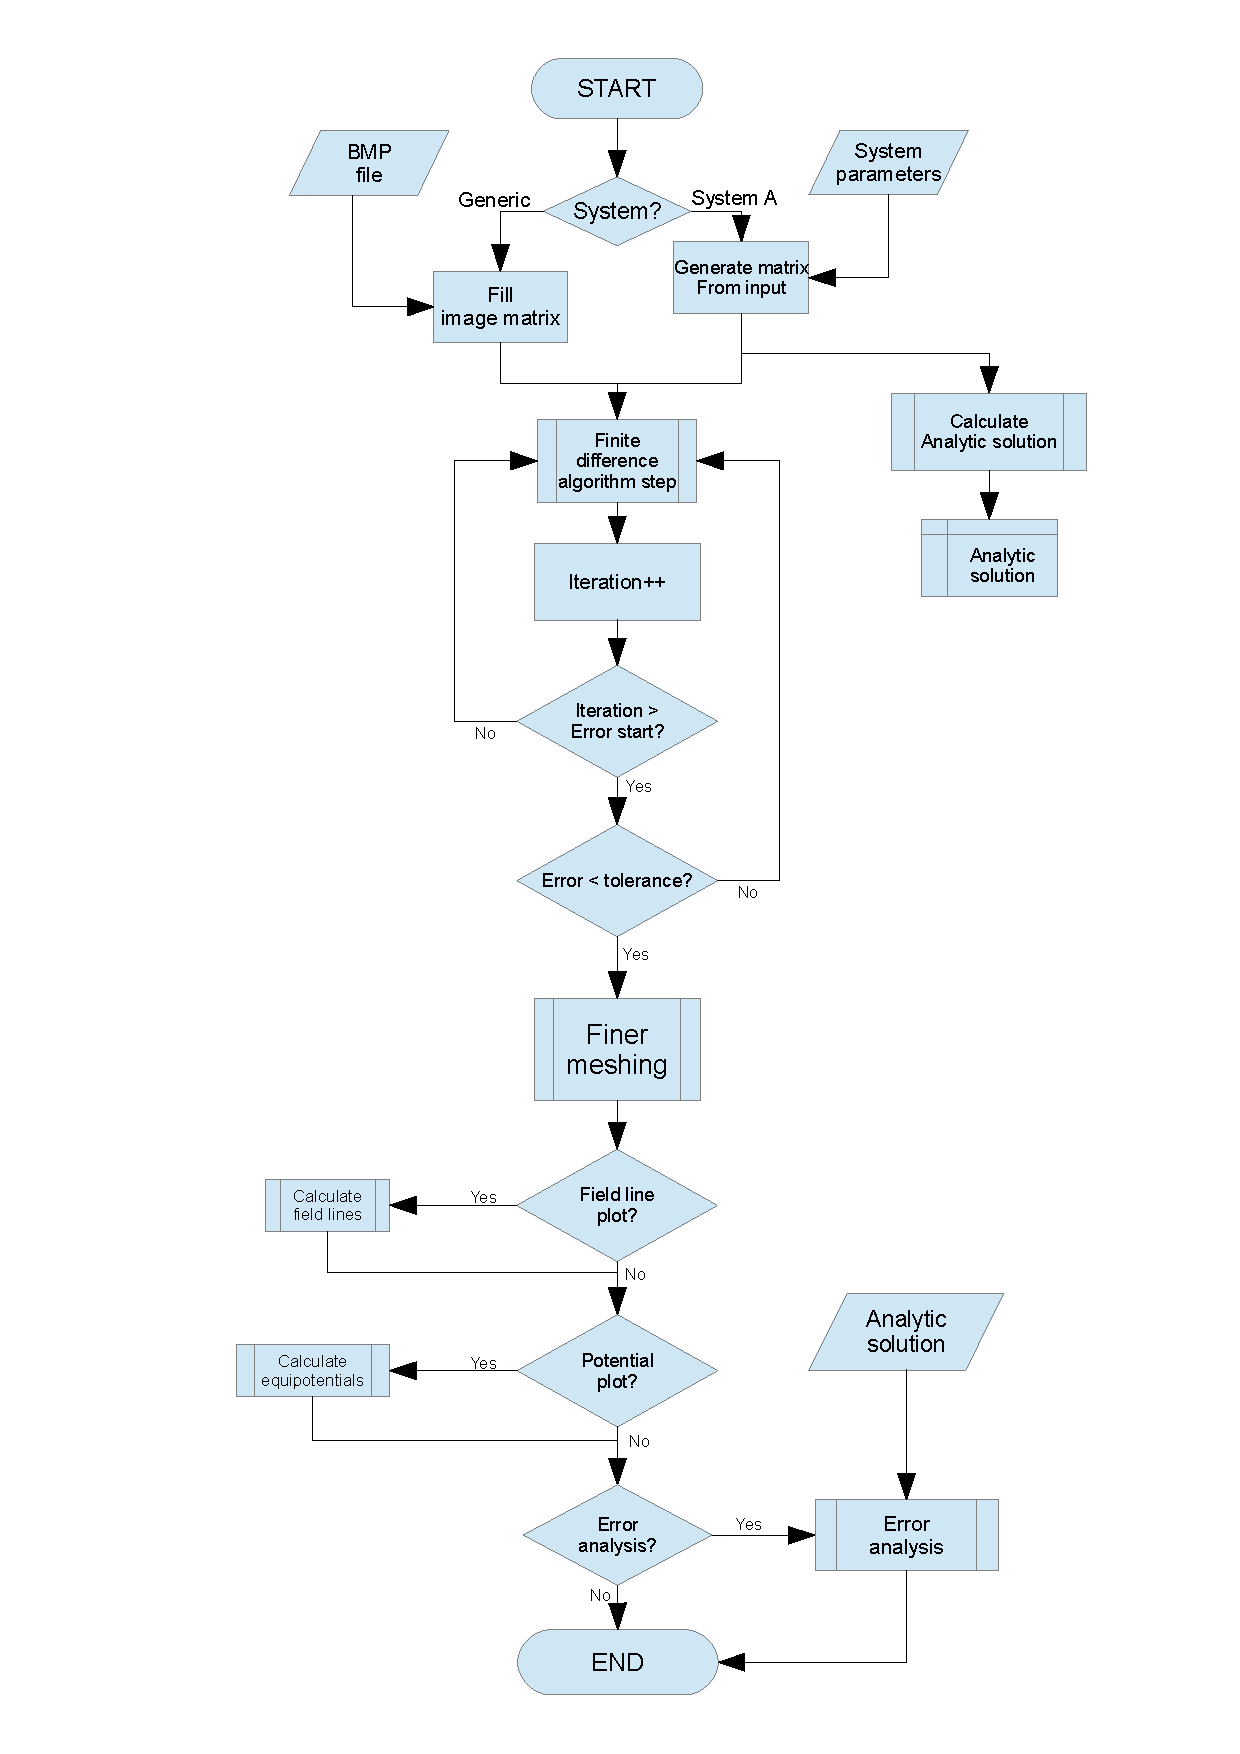
\includegraphics[width=13cm]{progflow} 
%	\caption{Program Flow}
%	\label{fig:prog}
%\end{figure}

\section*{System B}

A pixelated drawing describing the components of the system, a bitmap, was passed to the program. Each pixel was then mapped to a matrix holding values between -1 and 1, to represent the voltages of the initial system. The matrix elements related to components, that is, conductors or charges, were not changed during the numerical procedure while the rest varied as the program run.

%\begin{figure}[h]
%	\centering
%	\includegraphics[width=7cm]{GPdiagram21} 
%	\caption{systemB}
%	\label{fig:systemB}
%\end{figure}

\section*{References}
\bibliographystyle{ieeetr}
\bibliography{Bibliography3rdYear}

\end{document}